\documentclass[12pt]{article}

% Font and text formatting packages
\usepackage{microtype} % Improved text alignment and spacing
\usepackage[bitstream-charter]{mathdesign}
\usepackage{XCharter} % XCharter font
\usepackage[scaled]{beramono} % Monospaced font styling
% \usepackage[italic]{mathastext} % Italicizes math in text font for consistency

% Conditional checking
\usepackage{etoolbox}

% Enhanced typography
\usepackage[normalem]{ulem} % Underlining
\usepackage{contour} % Outline text (used with \contour command)
\usepackage{xpatch} % Enables patching commmands for typographical modifications
\usepackage{bm} % Italic bold

% Scientific notation and chemical formulas
\usepackage[version=4]{mhchem} % For chemical notation
\usepackage{siunitx} % Consistent handling of units

% Graphics
\usepackage{graphicx} % Essential for including images
\usepackage{subcaption} % Subfigures and subcaptions
\graphicspath{{./images/}} % Path for images directory

% Document layout
\usepackage[margin=1in]{geometry} % 1-inch margins
\usepackage{multicol} % Multi-column layouts

% Custom captions formatting
\usepackage{caption}
\DeclareCaptionFormat{custom}{\textbf{#1.} #3}
\captionsetup{format=custom}


\usepackage{csquotes} % Recommended for quotes in citations
\usepackage[style=apa, backend=biber]{biblatex} % APA style citations
\addbibresource{references.bib} % Reference file


% Custom underlining with contour effect
\contourlength{1.7pt} % Default contour length
\NewDocumentCommand{\ul}{O{2.62pt} O{0.45pt} O{1.5pt} m}{%
  \begingroup%
  \renewcommand\ULdepth{#1}%
  \renewcommand\ULthickness{#2}%
  \contourlength{#3}%
  \uline{\phantom{#4}}\llap{\contour*{white}{#4}}%
  \endgroup%
}

% Additional custom commands
\def\code#1{\texttt{#1}} % Inline code styling
\newcommand{\goldenRatio}{1.6180} % Golden ratio constant
\newcommand{\inverseGoldenRatio}{0.6180} % Inverse golden ratio constant

% Define automatic kerning for footnotes next to punctuation
\makeatletter
\xpatchcmd{\@makefnmark}{\hss}{\kern-0.5em\hss}{}{}
\makeatother

% Automatic extra spacing around em-dashes
\xpretocmd{\textemdash}{\hspace{0.1em}}{}{}
\xapptocmd{\textemdash}{\hspace{0.1em}}{}{}

\title{Temperature Effects on Phosphor Fluorescence Lifetime}
\date{September 16, 2024}
\author{\ul{Micah Hillman} \and Cordney Nash}

\begin{document}
  \maketitle

  \section*{Introduction}{
    Europium-doped phosphor compounds can exhibit temperature-dependent flourescence lifetimes for certain emission lines. In europium-doped lanthanum oxysulfide (\ce{La2O2S{:}Eu}), the variable overlap of a charge-transfer (CT) state with the \ce{^{5}D_{i}} energy levels leads to an increased availability of non-radiative de-excitation pathways as temperature is increased. For lower temperatures, the CT state becomes less available and radiative emission dominates, leading to longer fluorescence lifetimes. We measured fluorescence lifetimes for a sample of \ce{La2O2S{:}Eu} between \SI{-10}{\degreeCelsius} and \SI{100}{\degreeCelsius}, and observed a (linear/logarithmic) decrease in decay lifetimes for increasing temperatures.
  }

  \section*{Methods}{

  \begin{figure}[ht]
    \centering
    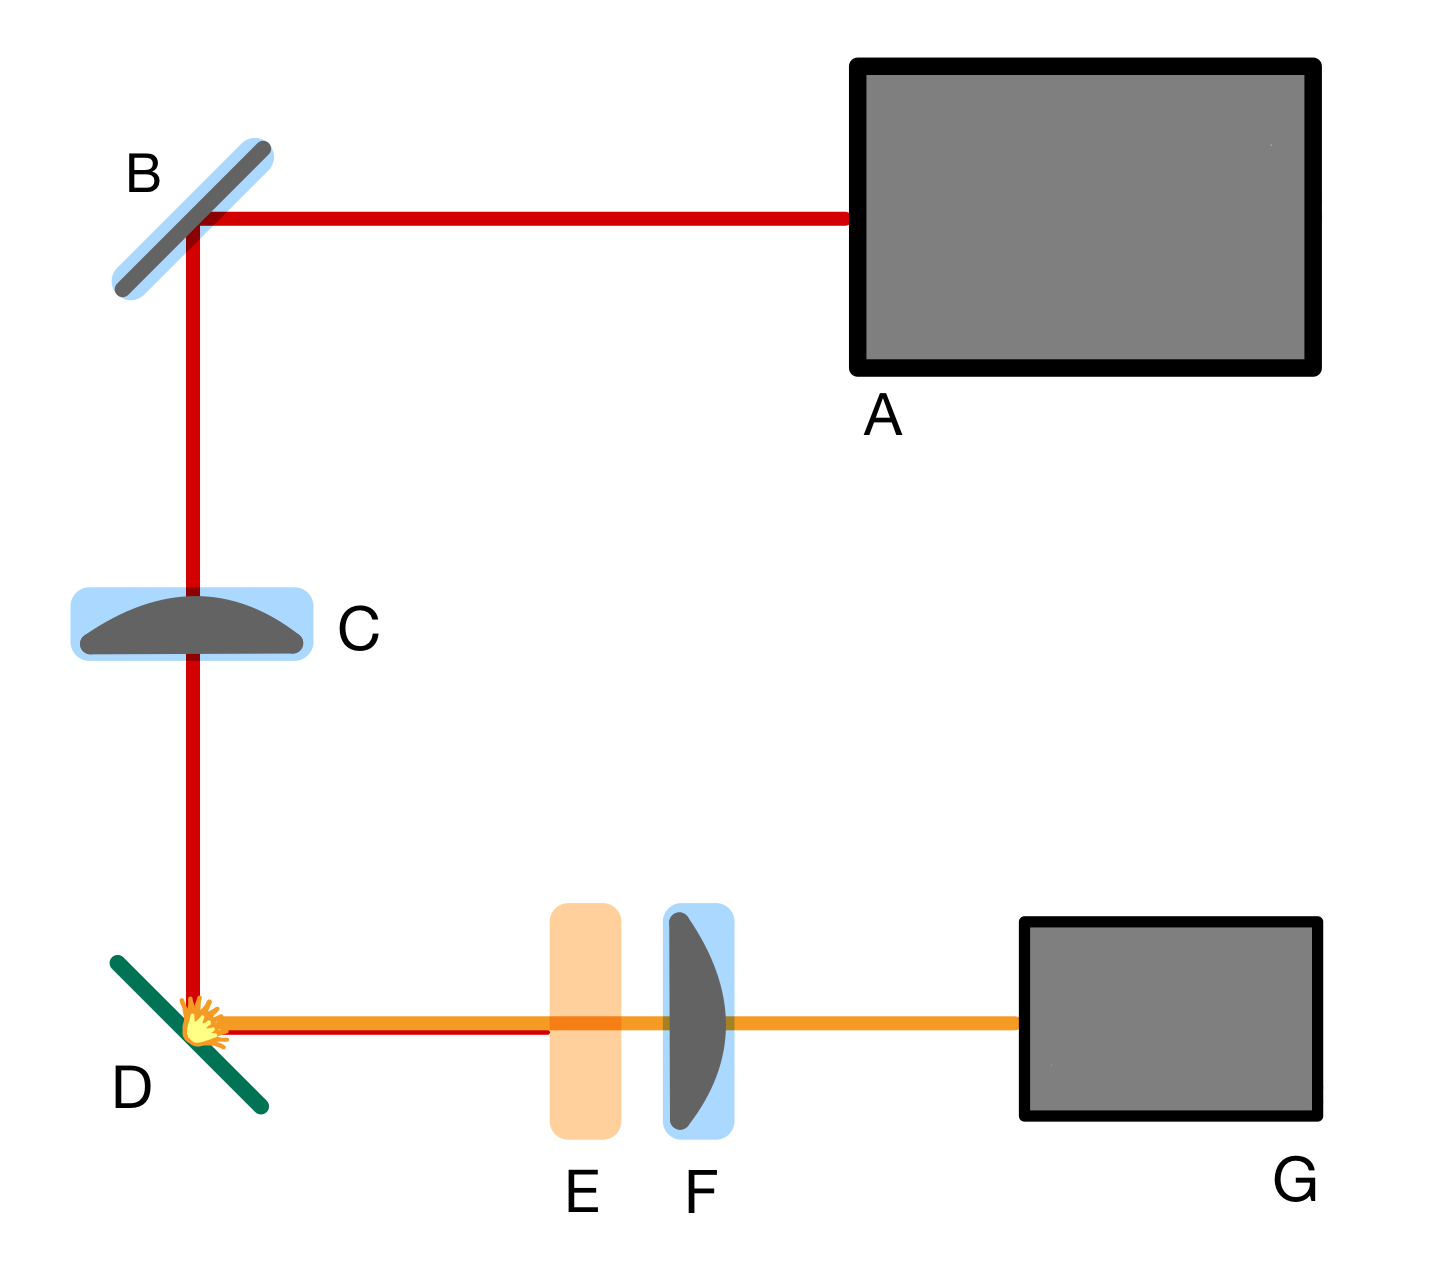
\includegraphics[width=\inverseGoldenRatio\linewidth]{experiment_diagram}
    \caption{A diagrammatic representation of the experimental setup.}\label{fig:setup}
  \end{figure}

    To modulate its temperature, the phosphor sample was mounted on a Peltier device attached to a manually-variable current source (\textbf{Figure~\ref*{fig:setup},~\(\bf{D}\)}). Focused light from a pulsing laser diode (\(\bf{A}\)) was reflected (\(\bf{B}\)) and focused (\(\bf{C}\)) on the surface of the sample, causing fluorescence at the \SI{514}{\nm}, \ce{^{5}D2} emission line (among others). Fluoresced light was then band-passed (\(\bf{E}\)) and focused (\(\bf{F}\)) into a photomultiplier tube (PMT) (\(\bf{G}\)). The PMT-amplified fluorescence response signal was then passed with the original impulse signal to be overlayed on a digital oscilloscope for data collection.
    
    After setting the pulse width of the laser diode to approximately \SI{1}{\micro\second}, we began varying the current supplied to the Peltier device to set the temperature at approximate steps of \SI{10}{\degreeCelsius} ranging from \SI{-10}{\degreeCelsius} to \SI{100}{\degreeCelsius}. Three snapshots of oscilloscope data were collected at each increment, where the oscilloscope timing window was variably tuned to meet the following specifications:
      
      \begin{enumerate}
        \item maximize timing resolution by including as many non-zero response values as possible, and
        \item include information about the fluorescence response's offset prior to the laser impulse (for offset subtraction during analysis).
      \end{enumerate}
    
    
  }

  \section*{Results}{
    \lipsum[1]
  }

\end{document}
